\hypertarget{chip__info_8h}{}\section{/var/www/html/\+S\+J\+S\+U-\/\+D\+E\+V-\/\+Linux/firmware/default/lib/\+L0\+\_\+\+Low\+Level/chip\+\_\+info.h File Reference}
\label{chip__info_8h}\index{/var/www/html/\+S\+J\+S\+U-\/\+D\+E\+V-\/\+Linux/firmware/default/lib/\+L0\+\_\+\+Low\+Level/chip\+\_\+info.\+h@{/var/www/html/\+S\+J\+S\+U-\/\+D\+E\+V-\/\+Linux/firmware/default/lib/\+L0\+\_\+\+Low\+Level/chip\+\_\+info.\+h}}


Provides the chip programming info.  


{\ttfamily \#include $<$stdint.\+h$>$}\\*
{\ttfamily \#include $<$string.\+h$>$}\\*
Include dependency graph for chip\+\_\+info.\+h\+:\nopagebreak
\begin{figure}[H]
\begin{center}
\leavevmode
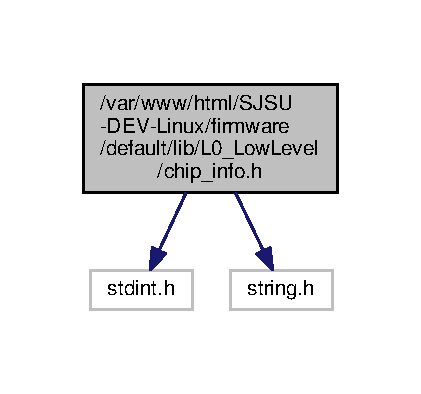
\includegraphics[width=202pt]{d0/dd1/chip__info_8h__incl}
\end{center}
\end{figure}


\subsection{Detailed Description}
Provides the chip programming info. 

This file is meant to have \char`\"{}magic\char`\"{} code so users cannot easily manipulate the number of times the chip has been programmed.

Though on the other hand, anyone with bootloader experience can break-\/in, but probably not young students muahaha \+:D 